\subsection{基于TEE的推测性加密}
\label{subsec:sgxdedup-encryption}

在获得会话密钥(\S\ref{subsec:sgxdedup-key-management})之后,密钥安全区与每个客户端建立安全信道,以在消息锁加密密钥生成过程中保护传输的明文数据块指纹/数据块加密密钥(\S\ref{subsec:sgxdedup-arch} )。然而,为了管理安全信道,密钥安全区需要付出高昂的加密/解密成本,且随着客户端数量增加,管理成本逐步提升。\sysnameS 在密钥安全区中使用推测性加密\textit{(Speculative Encryption)}\cite{eduardo2019Speculative}增强了安全信道管理,减轻了密钥安全区的在线加密/解密开销。

\paragraph*{推测性加密。}推测加密\cite{eduardo2019Speculative}采用计数器模式\textit{(CTR)}\cite{counter}进行数据加解密,在离线过程中预先计算加解密掩码,而在在线过程中仅使用加解密掩码与数据进行异或操作,以减少在线加解密过程中的计算开销。

具体来说,为了加密明文$M$,首先将$M$划分为一系列明文数据块$b_1、b_2、\ldots、b_m$(例如,在AES中将每个块的大小固定为16字节)。对于每个客户端,选择一个唯一的随机数\textit{nonce} $\theta$(只被使用一次的任意或非重复的随机数值)。然后,计算第$i$个明文数据块的掩码\textit{(Mask)}为$e_i = {\bf E}(K, \theta || i)$,其中${\bf E}()$是对称加密函数,$K$是密钥,$i$是计数器(\textit{Counter},用于计数器模式加解密),‘$||$’是连接运算符。最后,计算每个密文数据块$c_i = e_i \oplus b_i $,其中$\oplus$是按位异或运算符,并整合形成完整密文$C = c_1 || c_2 || \ldots || c_m$。为了解密密文,推测性加密技术如加密过程一样,为每个密文块生成掩码$e_i$,并通过$b_i = e_i \oplus c_i $解密得到相应的明文块,最终整合形成完整明文$M = b_1 || b_2 || \ldots || b_m$。由于掩码生成步骤独立于每个目标明文/密文的生成,推测性加密可以在离线时预先计算加解密掩码,然后应用轻量级异或操作进行在线加密/解密。

\begin{figure}[!htb]
    \centering
    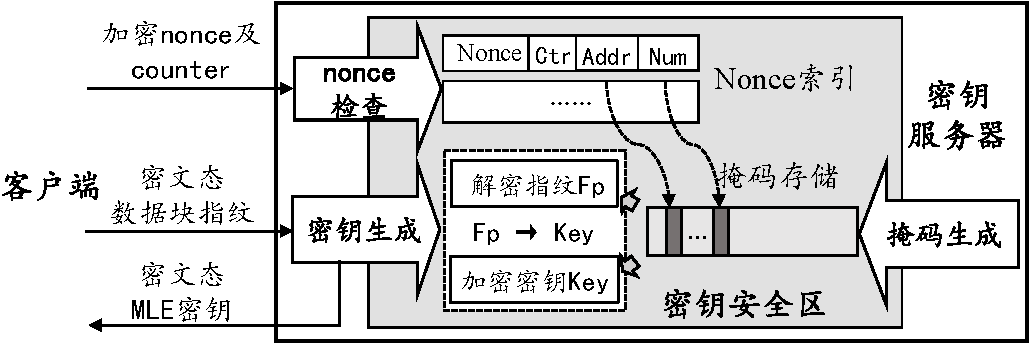
\includegraphics[width=0.9\textwidth]{pic/sgxdedup/key-enclave-arch.pdf}
    \caption{基于TEE的推测性加密概述}
    \label{fig:sgxdedup-SpecEnc}
\end{figure}

\paragraph*{与TEE的整合。}要在\sysnameS 中实现推测性加密,本文需要解决多客户端的nonce管理问题。在计数器模式加密中,唯一的nonce充当不可预测的“一次性填充”,使得加密输出看起来是随机的\cite{counter}。如果多个客户端使用计数器模式加密,则需要在每个客户端的加解密操作中关联一个唯一的nonce。但是,由于不同的客户端之间是隔离的,因此很难确保为客户端关联的nonce是唯一的。

为了确保nonce的唯一性,\sysnameS 在密钥安全区中管理一个集中的键值对(Key-value)结构,称为\textit{nonce}索引。 nonce索引的每个条目将存储的nonce(默认大小为12字节)映射到三个字段:其对应的计数器(4字节)、相应的加解密掩码存储的起始地址(8字节)和可用加解密掩码的数量(4字节)。此外,\sysnameS 实现了nonce检查安全区内调用(\textit{nonce checks ECall})。如图~\ref{fig:sgxdedup-SpecEnc}所示,它可以被密钥服务器调用,以将每个客户端提交的nonce与之前存储在nonce索引中的nonce进行比较,并在发现重复nonce时要求客户端重新选择nonce。在安全区内存大小限制下,本文使用3\,MiB(\sysnameS 的默认值)安全区内存空间管理多达112,000个客户端的信息(假设每个客户端仅一个nonce)。

\sysnameS 使用推测性加密在客户端和密钥安全区之间建立安全信道,以保护消息锁加密密钥生成。在建立安全信道的过程中,客户端若为第一次启动,则随机挑选加密nonce $\theta$,并将计数器$i$置为0;若客户端非第一次启动(即本地保存有旧的nonce $\theta$和计数器$i$)则使用已有nonce $\theta$和计数器i进行加解密操作。

具体来说,客户端使用最新的会话密钥(\S\ref{subsec:sgxdedup-key-management})加密$\theta$和$i$,根据生成的密文计算消息验证码(MAC),并将密文和MAC提交给密钥服务器。这里,本文采用先加密后签名机制(\textit{Encrypt-then-MAC})\cite{bellare2000Authenticated},密钥安全区通过检查密文和MAC来检测客户端是否使用过期的会话密钥,以阻止未授权客户端访问密钥生成服务。密钥服务器随即发出nonce检查安全区内部调用(Nonce checking Ecall),该安全区内部调用将客户端上传的密文和MAC作为输入,在密钥安全区内解密$\theta$和$i$,并使用nonce索引检查解密后的$\theta$和$i$,检查的结果可分为如下三种情况:

\begin{itemize}[leftmargin=0em]
    \item \textbf{情况1:$\theta$是重复的且计数器$i = 0$。}表示该nonce已被其他客户端使用,则通过密钥服务器发送通知,要求客户端重新选择新的nonce。
    \item \textbf{情况2:$\theta$是重复的并且计数器$i \neq 0$。}表明该nonce已被存储,如果该nonce对应的加解密掩码已经预先计算完成(可用)则进行标记,并通过密钥服务器通知客户端开始执行密钥生成。
    \item \textbf{情况3:$\theta$是不重复的。}即,没有已保存的nonce和该nonce相同,则将该nonce添加到nonce索引中,并通过密钥服务器通知客户端开始执行密钥生成。
\end{itemize}

对于情况2和3,密钥安全区接受密钥生成请求,并要求客户端传输数据块指纹以生成消息锁加密密钥(\S\ref{subsec:sgxdedup-arch})。具体来说,客户端根据$\theta$和$i$对数据块指纹进行加密,并上​​传结果;在加密每个数据块指纹后,客户端将计数器$i$自增1以防止重放攻击。如图~\ref{fig:sgxdedup-SpecEnc}所示,密钥服务器发出密钥生成安全区内部调用(\textit{key generation ECall})来处理加密的数据块指纹。密钥安全区首先检查是否为当前客户端离线生成了加解密掩码。如果找到(即,情况2),密钥安全区使用离线生成的掩码来解密指纹并加密生成的消息锁加密密钥。否则(即,情况3),密钥安全区在线计算加解密掩码以进行解密收到的指纹并加密生成的消息锁加密密钥。

\paragraph*{加解密掩码离线计算。}为了加速密钥安全区在线加密/解密,当应用新的会话密钥(使得所有现有离线生成的加解密掩码失效)或客户端在至少一个离线计算的加解密掩码被使用且停止密钥生成请求后,密钥服务器通过掩码生成安全区内部调用(\textit{Mask generation ECall},图~\ref{fig:sgxdedup-SpecEnc})要求密钥安全区根据预设离线计算掩码对应客户端数据量为访问频率最高的多个nonce生成对应的掩码(例如,在\sysnameS 中默认为三个)并将生成的掩码放入掩码存储区。默认情况下,本文将掩码存储区配置为最大 90\,MiB。假设每个掩码占用16个字节,重复数据删除系统中平均数据块大小为8\,KiB,每个指纹的消息锁加密密钥生成使用四个掩码(两个用于解密32字节指纹,另外两个用于加密生成的32字节消息锁加密密钥)。当掩码存储区被全部利用时,其中的加解密掩码可用于处理多达11.25\,GiB原始文件数据所产生的数据块指纹。
